\documentclass{article}

\usepackage{tikz}
\usetikzlibrary{arrows.meta}

\begin{document}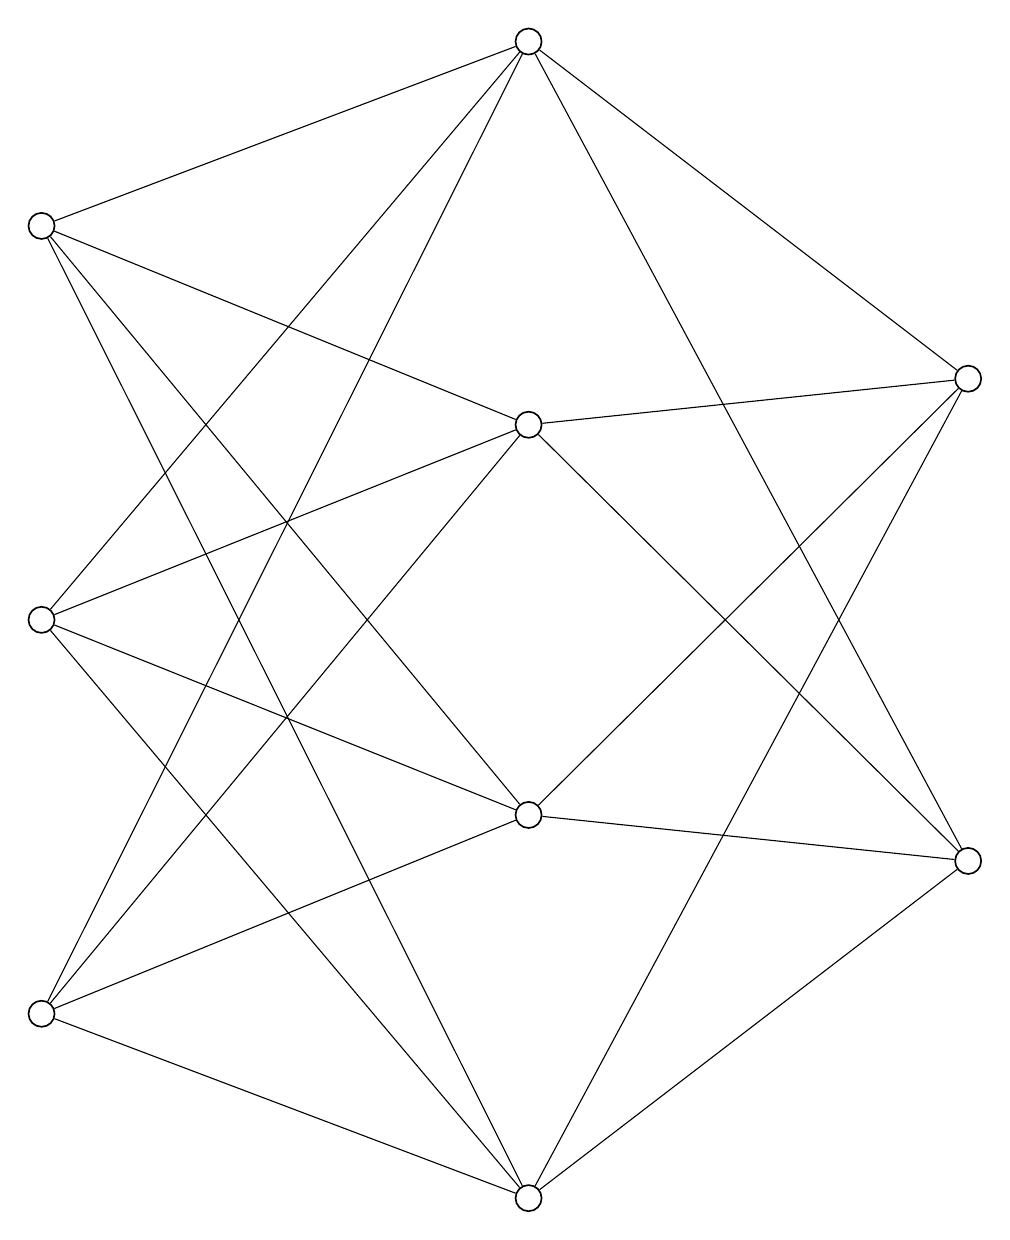
\begin{tikzpicture}[>={Latex},
  default/.style={draw=black, semithick, solid, fill=white, solid},
  every loop/.style={looseness=16}]
\node[default, circle] (L1A) at (-5.364084, 0.00006) {};
\node[default, circle] (L1B) at (-5.364084, -5.002772) {};
\node[default, circle] (L1C) at (-5.364084, 5.002878) {};
\node[default, circle] (L2A) at (0.82117, 2.477616) {};
\node[default, circle] (L2B) at (0.82117, 7.34427) {};
\node[default, circle] (L2C) at (0.82117, -7.344404) {};
\node[default, circle] (L2D) at (0.82117, -2.477882) {};
\node[default, circle] (L3A) at (6.403786, -3.061911) {};
\node[default, circle] (L3B) at (6.403786, 3.062145) {};
\draw [] (L1A) -- (L2A) ;
\draw [] (L1A) -- (L2B) ;
\draw [] (L1A) -- (L2C) ;
\draw [] (L1A) -- (L2D) ;
\draw [] (L1B) -- (L2A) ;
\draw [] (L1B) -- (L2B) ;
\draw [] (L1B) -- (L2C) ;
\draw [] (L1B) -- (L2D) ;
\draw [] (L1C) -- (L2A) ;
\draw [] (L1C) -- (L2B) ;
\draw [] (L1C) -- (L2C) ;
\draw [] (L1C) -- (L2D) ;
\draw [] (L2A) -- (L3A) ;
\draw [] (L2A) -- (L3B) ;
\draw [] (L2B) -- (L3A) ;
\draw [] (L2B) -- (L3B) ;
\draw [] (L2C) -- (L3A) ;
\draw [] (L2C) -- (L3B) ;
\draw [] (L2D) -- (L3A) ;
\draw [] (L2D) -- (L3B) ;
\end{tikzpicture}
\end{document}
